\documentclass[11pt,a4paper]{article}
\usepackage{amsmath,amsthm,amsfonts,amssymb,amscd}
\usepackage{enumerate} 
\usepackage{physics}
\usepackage{enumerate}
\usepackage{fancyhdr}
 \usepackage{hyperref}
\hypersetup{colorlinks,
    linkcolor=blue,
    citecolor=blue,      
    urlcolor=blue,
}
\usepackage{graphicx}


\oddsidemargin0.1cm 
\evensidemargin0.8cm
\textheight22.7cm 
\textwidth15cm \topmargin-0.5cm

\newtheorem{theorem}{Theorem}[section]
\newtheorem{lemma}[theorem]{Lemma}

\usepackage{listings}
\usepackage{xcolor}

\definecolor{codegreen}{rgb}{0,0.6,0}
\definecolor{codegray}{rgb}{0.5,0.5,0.5}
\definecolor{codepurple}{rgb}{0.58,0,0.82}
\definecolor{backcolour}{rgb}{0.95,0.95,0.92}

\lstdefinestyle{mystyle}{
    backgroundcolor=\color{backcolour},   
    commentstyle=\color{codegreen},
    keywordstyle=\color{magenta},
    numberstyle=\tiny\color{codegray},
    stringstyle=\color{codepurple},
    basicstyle=\ttfamily\footnotesize,
    breakatwhitespace=false,         
    breaklines=true,                 
    captionpos=b,                    
    keepspaces=true,                 
    numbers=left,                    
    numbersep=5pt,                  
    showspaces=false,                
    showstringspaces=false,
    showtabs=false,                  
    tabsize=2
}

\lstset{style=mystyle}

\newcommand{\silvia}[1]{{ {\color{blue}{(silvia)~#1}}}}
\newcommand{\grace}[1]{{ {\color{purple}{(grace)~#1}}}}

\newcommand{\MultiSet}{\mathrm{MultiSet}}
\newcommand{\len}{\mathrm{len}}
\newcommand{\din}{\texttt{d\_in}}
\newcommand{\dout}{\texttt{d\_out}}
\newcommand{\T}{\texttt{T} }
\newcommand{\F}{\texttt{F} }
\newcommand{\Relation}{\texttt{Relation}}
\newcommand{\X}{\mathcal{X}}
\newcommand{\Y}{\mathcal{Y}}
\newcommand{\True}{\texttt{True}}
\newcommand{\False}{\texttt{False}}
\newcommand{\clamp}{\texttt{clamp}}
\newcommand{\function}{\texttt{function}}
\newcommand{\float}{\texttt{float }}
\newcommand{\questionc}[1]{\textcolor{red}{\textbf{Question:} #1}}


\title{Privacy Proofs for OpenDP: Impute Constant Transformation}
\author{Grace Tian}
\date{Summer 2021}
\begin{document}


\maketitle
\tableofcontents

\section{Algorithm Implementation}
\subsection{Code in Rust}
The current OpenDP library contains the \texttt{make\_impute\_constant} function implementing the impute constant function. This is defined in lines 62-75 of the file \texttt{impute.rs} in the Git repository (\url{https://github.com/opendp/opendp/blob/21-impute/rust/opendp/src/trans/impute.rs#L62-L75}).

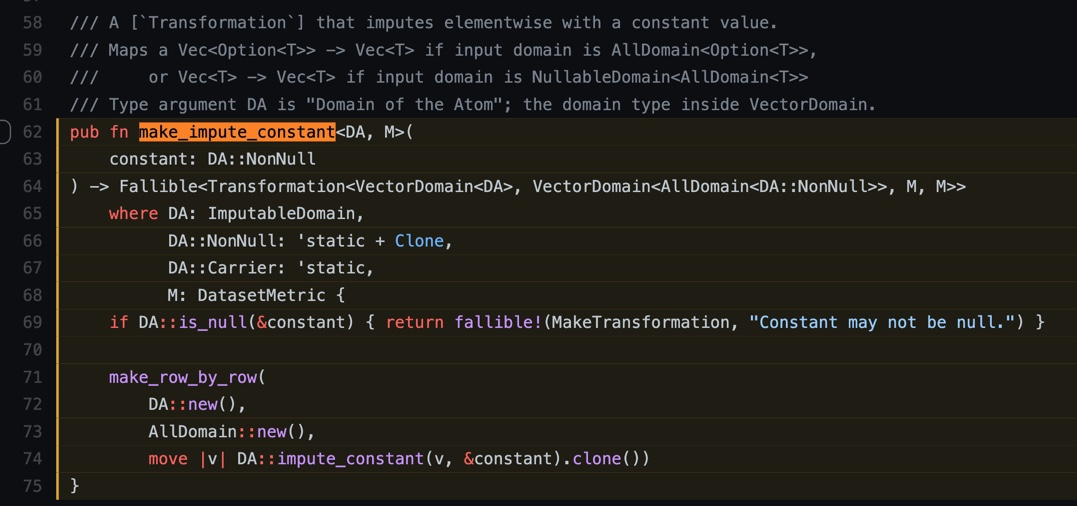
\includegraphics[width=\textwidth]{make_impute_constant.jpg}


\subsection{Pseudo Code in Python}\label{sec:pseudocode}

\subsubsection*{Preconditions}
To ensure the correctness of the output, we require the following preconditions:

\begin{itemize}
    \item \textbf{User-specified types:}
    \begin{itemize}
        \item Variable \texttt{\texttt{constant}} must be of type \texttt{DA::Imputed}
        \item Type \texttt{DA} is a domain with \texttt{ImputableDomain} trait. % Unless the null method is defined, this means that \texttt{DA} is either \texttt{OptionNullDomain<AllDomain<T>>} or \texttt{InherentNullDomain<AllDomain<T>>}.
        \item \texttt{DA::Imputed} must have traits \texttt{Clone}
    \end{itemize}
\end{itemize}

\subsubsection*{Postconditions}

\begin{itemize}
    \item Either a valid \texttt{Transformation} is returned or an error is returned.
    \item \grace{Should I also say that \texttt{impute\_constant} must satisfy the preconditions of make row by row? (See pseudo code \ref{line:row-transform}.) That is, \texttt{impute\_constant} must be a pure function?}
\end{itemize}


\begin{lstlisting}[language=Python,  escapechar=|]
def make_impute_constant(constant : DA::Imputed):
    # instead of VectorDomain(DA), we add ::new() to get a new instance of DA. This is because DA has the ImputableDomain trait.
    input_domain = VectorDomain(DA::new())
    output_domain = VectorDomain(AllDomain(DA::Imputed))
    input_metric = SymmetricDistance()
    output_metric = SymmetricDistance()
    
    assert(not constant.is_null); # not DA::is_null(constant) |\label{line:null}|

    def function(data: Vec[DA::Carrier]) -> Vec[DA::Imputed]: |\label{line:fn}|
        return list(map(DA::impute_constant, data)) |\label{line:map}|
        
    return make_row_by_row(input_domain, output_domain,DA::impute_constant) |\label{line:row-transform}|
\end{lstlisting}

\subsection{Proof}

\begin{lemma}[\texttt{DA::Imputed} contains \texttt{null}] \label{lemma:Imputed}
A \texttt{var} of type \texttt{DA::Imputed} can be of type \texttt{null}.
\end{lemma}
\begin{proof}
Let the domain of atom variable \texttt{DA} be \texttt{InherentNullDomain<AllDomain<f64>>}. Recall that \texttt{InherentNullDomain} exists for types that can represent null inherently in the carrier type. Then the type $$\texttt{DA::Imputed == InherentNullDomain<AllDomain<f64>>::Imputed == f64}.$$ The latter holds because in the \texttt{InherentNullDomain} implementation in the rust code \url{https://github.com/opendp/opendp/blob/main/rust/opendp/src/trans/impute.rs#L48-L56}, the \texttt{type Imputed = Self::Carrier}. The \texttt{Carrier} of \texttt{VectorDomain<AllDomain<T>>} has type \texttt{T}, so in this case the \texttt{::Carrier} is type \texttt{f64}.

Therefore \texttt{var} is also of type \texttt{f64}. \texttt{f64} can contain \texttt{null} values, so we are done.
\end{proof}

\begin{lemma}[Precondition for row transform]\label{lemma:pure-fn}
\texttt{make\_impute\_constant} satisfies the preconditions of \texttt{make\_row\_by\_row}. That is, the atom function \texttt{impute\_constant} in pseudo code line \ref{line:atom-fn} is a pure function. 
\end{lemma}
\begin{proof}
We reference the examples in Definition 3.4 in the proofs definition document for the definition of a pure function, and later as a check list to verify the properties of a pure function hold. To verify whether \texttt{impute\_constant} is a pure function, it must satisfy the following properties:
\begin{enumerate}
    \item The function return values are identical for identical arguments.
    \item The function application has no side effects.
\end{enumerate}

The first property is satisfied because there is no static variable defined within \\\texttt{make\_impute\_constant}, no mutable reference argument, no return value of an input stream, all of which could potentially cause different function outputs for inputs. The return value stays the same for the same input to \texttt{impute\_constant} since constant is hard wired into the function and never changed in the code. 

The second property is satisfied because the local static variables and non-local variables are unchanged, and there are no mutable reference arguments or input/output streams called within the \texttt{impute\_constant}.
\end{proof}

\begin{theorem}
For every setting of the input parameters \texttt{constant} to \texttt{make\_impute\_constant} such that the given preconditions hold, the transformation returned by \texttt{make\_impute\_constant} has the following properties:
\begin{enumerate}
    \item \textup{(Appropriate output domain).} If vector $v$ is in the \texttt{input\_domain}, then \texttt{function(v)} is in the \texttt{output\_domain}.
    \item \textup{(Domain-Metric Compatibility).} The domain \texttt{input\_domain} matches one of the possible domains listed in the definition of \texttt{input\_metric}, and likewise \texttt{output\_domain} matches one of the possible domains listed in the definition of \texttt{output\_metric}.
    \item \textup{(Stability Guarantee).} For every pair of elements $v, w$ in \texttt{input\_domain} and for every pair $(\din, \dout)$, where $\din$ is of the associated type for \texttt{input\_metric} and $\dout$ is the associated type for \texttt{output\_metric}, if $v,w$ are $d_{in}$-close under \texttt{input\_metric} and $\Relation(\din, \dout) = \True$, then $\function(v), \function(w)$ are $d_{out}$-close under \texttt{output\_metric}.
\end{enumerate}
\end{theorem}
\begin{proof}
\begin{enumerate}

\item \textbf{(Appropriate output domain).} 

In the case of \texttt{make\_impute\_constant}, this corresponds to showing that for every vector $v$ of elements of type \texttt{DA::Carrier},  \texttt{function}$(v)$ is a vector of elements of type \texttt{DA::Imputed}. We can also say that \texttt{function}$(v)$ is a vector of elements that does not contain any \texttt{Imputed} values.

The $\function(v)$ has type \texttt{Vec[DA::Imputed]} follows from the assumption that element $v$ is in \texttt{input\_domain} and from the type signature of \texttt{function} in line~\ref{line:fn} of the pseudocode (Section~\ref{sec:pseudocode}). The type signature takes in an element of type \texttt{Vec[DA::Carrier]} and returns an element of type \texttt{Vec[DA::Imputed]}. If the Rust code compiles correctly, then the type correctness follows from the definition of the type signature enforced by Rust. Otherwise, the code will halt at compile time.

The type signature is not a sufficient check, since by Lemma \ref{lemma:Imputed}, the function's output type can represent a value (e.g. \texttt{float nan}) that is not a member in the \texttt{output\_domain}. \grace{How do I clarify that the output domain \\ \texttt{VectorDomain(AllDomain(DA::Imputed))} should actually contain NO NULLS? The code seems too loose because in Lemma 1.1 we just showed that \texttt{DA::Imputed} can contain null values.} To ensure that function returns the appropriate output domain at run time, we must ensure that at run time the \texttt{function}$(v)$ is not null. To do so, we must check whether the \texttt{constant} is not null.

Since the \texttt{constant} has type \texttt{DA::Imputed} and \texttt{DA::Imputed} may itself be \texttt{f64} by Lemma \ref{lemma:Imputed}, without an extra check \texttt{constant} can be null. We must check whether \texttt{constant} is null because otherwise if \texttt{constant} is null, the user can nonsensically impute \texttt{null} entries in a vector with \texttt{null} value. 

We check whether the constant is null in pseudo code line \ref{line:null}, before it gets called in \texttt{function}. If \texttt{constant} is \texttt{null}, then the check raises a construction-time error, so the function is never run. Thus we are done.

\grace{I didn't use the fact that v is of type DA::Carrier; am I doing something wrong?}

\item \textbf{(Domain-metric compatibility).} The Symmetric distance is both the \texttt{input\_metric} and \texttt{output\_metric}. Symmetric distance is compatible with \texttt{VectorDomain(T)} for any generic type \texttt{T}, as stated in \href{https://www.overleaf.com/project/60d215bf90b337ac02200a99}{``List of definitions used in the pseudocode"}. The theorem holds because for \texttt{make\_impute\_constant}, the input domain is \texttt{VectorDomain(DA)} and the output domain is \texttt{VectorDomain(AllDomain(DA::Imputed))}. 

\item \textbf{(Stability guarantee).} Since \texttt{impute\_constant} calls a row transform in line \ref{line:row-transform} and satisfies the necessary preconditions in Lemma \ref{lemma:pure-fn}, the stability guarantee of \texttt{impute\_constant} follows from the stability guarantee of row transforms in \href{https://www.overleaf.com/2489843918kjvyyytkjfsg}{\texttt{make\_row\_by\_row}}. 

\end{enumerate}
\end{proof}

\end{document}
